\chapter{\#16: Traffic Congestion}

\section{Introduction}
 
For this task the transportation of packages over a network, more specifically the internet, will be modelled. To do this two approaches will be used. The first follows Arenas et al. \cite{hierarchical_traffic}. Here packages are generated at each time step with probability $p$ on a hierarchical tree network. These networks are characterised by $z$, the branching factor, and $m$, the number of layers. Every package gets assigned a random node as its destination and they are left to perform a random walk until they reach their destination. The probability to jump from node $i$ to $j$ is given by the \textit{quality of communication} $q_{ij}$:

\begin{equation}
    q_{ij} = \sqrt{k_{ij} k_{ji}}
\end{equation}

\noindent with $k_{ij}$ representing the capability of nodes $i$ and $j$ to communicate with each other.

\begin{equation}
    k_{ij} = \xi_{ij} f(n_i)
\end{equation}

\noindent $\xi_{ij}$ is a uniformly distributed random between [0,1]. In the first part of the paper $\xi_{ij} = 1$, which is used in this analysis. $f(n_i)$ will be used to describe congestion in the system, depending on the number of packages in node $i$ ($n_i$) at a given time step. Here we will use the following form:

\begin{equation}
    f(n) = 
    \begin{cases}
      1, & \text{for}\ n=0 \\
      n^{-\gamma}, & \text{for}\ n=1, 2, 3, ...
    \end{cases}
\end{equation}

\noindent If the probability to generate a package $p$ is not too high, the system should tend towards an equilibrium where package generation and delivery balance each other out.

The second approach by Echenique et al. \cite{optimal_routing}, \cite{optimal_routing2} uses a directed method to propagate the packages. Here the following Hamiltonian is introduced:

\begin{equation}
    H_i = hd_i - (1-h)c_i
\end{equation}

\noindent $d_i$ is the amount of hops required to go from node $i$ to the destination node. $c_i$ is the number of packets in queue on a given node. At every time step, only the top node of a queue is allowed to move, the rest have to wait. The probability for a node to move to the next is then given by:

\begin{equation}
    \Pi_i = \frac{e^{-\beta H_i}}{\sum_j e^{-\beta H_j}}
\end{equation}

For $h=1$ the packets follow the shortest path to their destination. For $h<1$ they start avoiding more congested nodes.

\section{Results}

Just like the previous task, quantities are averaged over 10 iterations. This task was plagued by long computation times and (for the second part) numerical instability. This means that the networks used are quite small with about 100 nodes. Still, a few results could be obtained. Let us first study the model by Arenas et al. \cite{hierarchical_traffic}. First, the behaviour of the model is tested by studying the influence of the parameter $p$, the probability of generating a package in a node. It can clearly be seen that for low values of $p$, equilibrium can be reached, whereas larger values result in a continuous increase of the number of packages.

\begin{figure}[H]
    \centering
    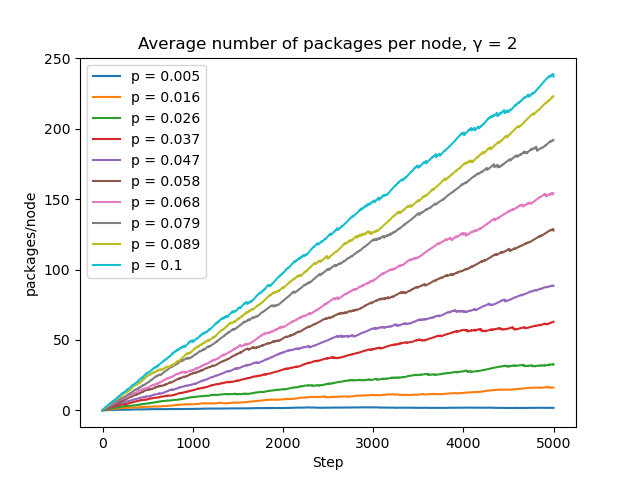
\includegraphics[width=0.75\linewidth]{images/gam_3_smallRange.png}
    \caption{\textit{Evolution of package numbers for different generation probabilities $p$}}
    \label{p_influence}
\end{figure}

Next, we can explore the influence of both the parameters $p$ and $\gamma$. After a set number of steps (about 3000) the size of deviations from the number of nodes at that point was calculated at each step and averaged out. This serves of a measure of whether or not a system has reached (or can reach) equilibrium. This is better than looking at the size of the system at the end of the simulation and comparing it to the value at a set point as fluctuations near the end might significantly influence this. 

\begin{figure}[H]
    \centering
    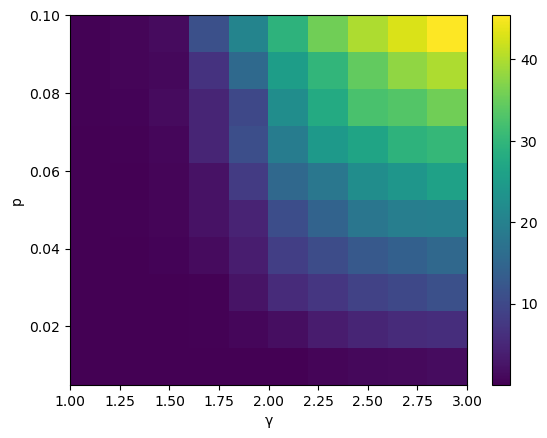
\includegraphics[width=0.7\linewidth]{images/parameter_space.png}
    \caption{\textit{Influence of both $p$ and $\gamma$. The colour bar represents the average size of fluctuations around the package number at a certain step. This package value is roughly where equilibrium starts for the lower combinations of $p$ and $\gamma$. The higher combinations result in divergence and will keep growing.}}
    \label{parameter_space}
\end{figure}

\noindent Next the dynamics on an ER network is studied. One would expect the ER network (with a high enough wiring probability) results in a lower number of packages at equilibrium. This is what is observed in Figure \ref{netw_comparison}.

\begin{figure}[H]
    \centering
    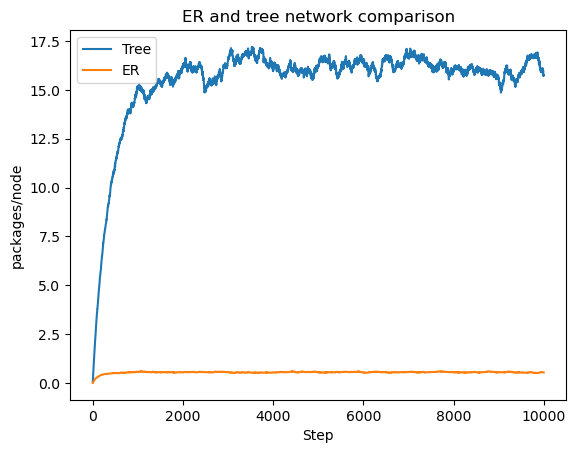
\includegraphics[width=0.7\linewidth]{images/netw_comparison.png}
    \caption{\textit{Comparison between the package dynamics on a tree and Erdös-Renyi network}}
    \label{netw_comparison}
\end{figure}

Finally the critical behaviour of this model was studied by using the analytical expression for $p_c$, the critical value for $p$:

\begin{equation}
    p_c = \frac{\sqrt{z}}{\frac{z(z^{m-1} - 1)^2}{z^m - 1} + 1}
\end{equation}

and the order parameter $\eta$ defined as $\eta = \frac{p-1}{p}$. The results are shown in Figure \ref{crit}. The results are not like those obtained in the paper. I am not sure what went wrong in my modelling.

\begin{figure}[H]
    \centering
    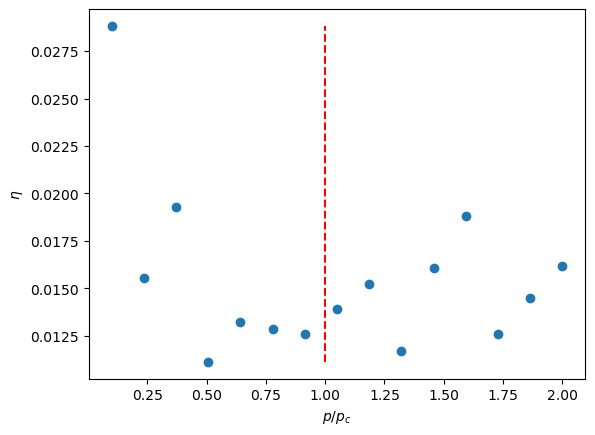
\includegraphics[width=0.5\linewidth]{images/critical_behaviour.png}
    \caption{\textit{Critical behaviour of the traffic model for z=3, m=5}}
    \label{crit}
\end{figure}

The network employed in the second model is the Barabási-Albert model. This method is giving ok results, but not fully compatible with the research papers. For congested networks one would expect the traffic aware scheme to perform better but it appears to not make a difference in my implementation. This is shown in Figure \ref{method2_evol}. The scaling with the number of initial packages seems reasonable as a lower density of packages allows for faster delivery.

\begin{figure}[H]
    \centering
    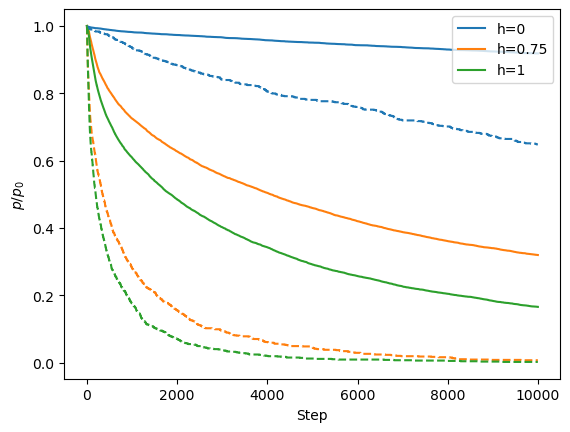
\includegraphics[width=0.5\linewidth]{images/method2_evol.png}
    \caption{\textit{Evolution of the number of packages normalised to the number at step 0 on a network of 1000 nodes. The full lines are for $10^4$ initial packages, dashed for $10^3$}}
    \label{method2_evol}
\end{figure}


\section{Runtime scaling}

As mentioned, the runtime was a large obstacle for this task. To measure its scaling with the system size the simulation code was run over just a single iteration (normally 10 would be done to average out fluctuations) for differing values of $z$ and a set value of $m = 4$. The results were then fitted with both an exponential $t = e^{\alpha z}$ and a power scaling fit $t = z^\beta$. The results are presented in Figure \ref{time_scaling}. From the fits the following values were found: $\alpha \approx 1.14$, $\beta \approx 4.05$. Extrapolating with these parameters we find that a system with branching factor $z = 10$ ($N = 1111$) would take 3 hrs (power function) or 24 hrs (exponential) for a single iteration.

\begin{figure}[H]
    \centering
    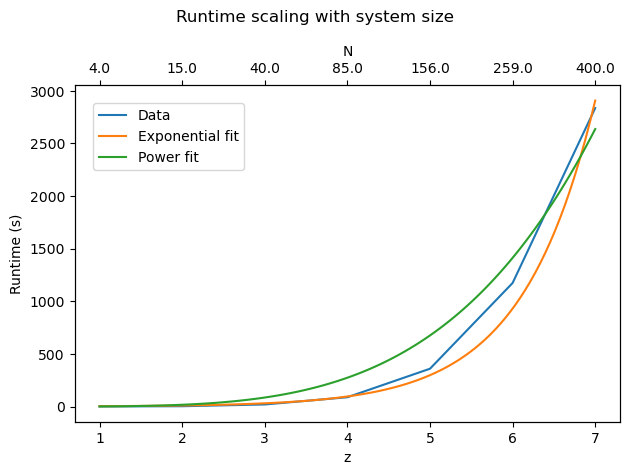
\includegraphics[width=0.8\linewidth]{images/time_scaling.png}
    \caption{\textit{Scaling of runtime of a single iteration for differing values of the branching factor $z$ with a fixed number of levels $m$}}
    \label{time_scaling}
\end{figure}


\newpage